\documentclass[border=10pt]{standalone}

\usepackage{tikz}
\usepackage{tikzsymbols}
\usetikzlibrary{calc,patterns,shapes.geometric}

\def\centerarc[#1](#2)(#3:#4:#5){\draw[#1] ($(#2)+({#5*cos(#3)},{#5*sin(#3)})$) arc (#3:#4:#5);}

\begin{document}
	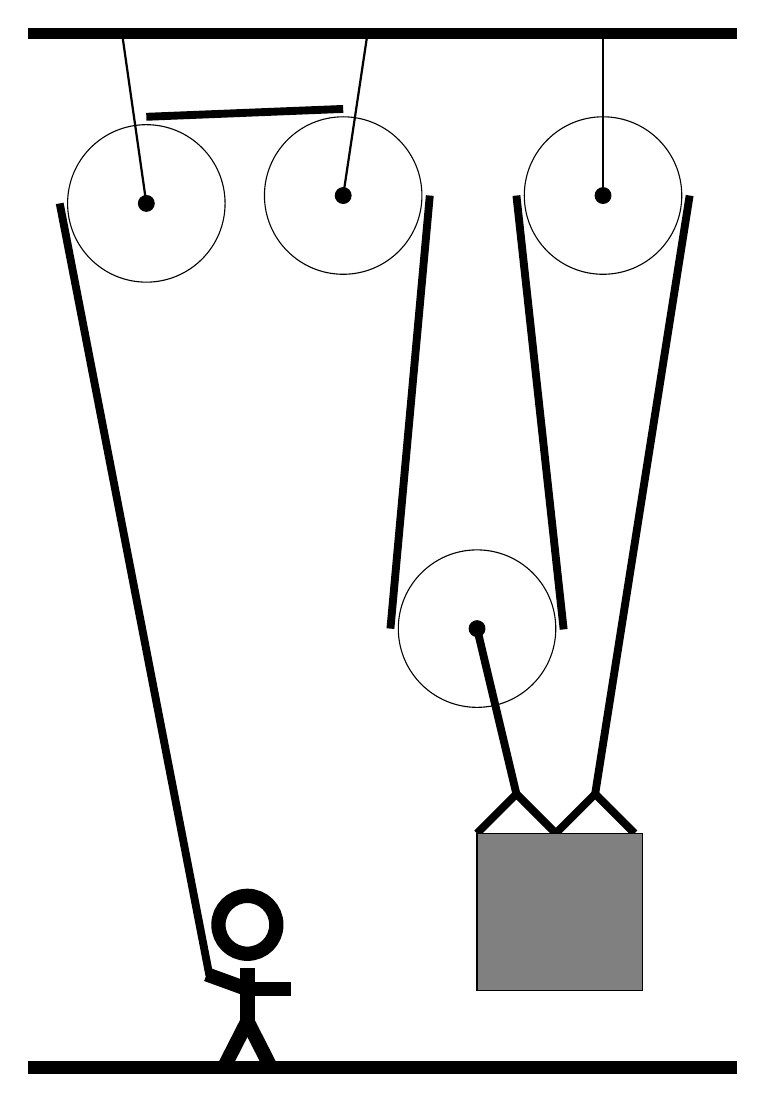
\begin{tikzpicture}
		%%%%% START %%%%%
		\draw[fill=black] (-3, 10) rectangle (6, 10.125);
		
		\draw (1, 8.0) circle (1);
		\draw[fill=black] (1, 8.0) circle (0.1);
		\draw[thick] (1, 8.0) -- (1.3, 10);
		
		\draw (4.3, 8.0) circle (1);
		\draw[fill=black] (4.3, 8.0) circle (0.1);
		\draw[thick] (4.3, 8.0) -- (4.3, 10);
		
		\draw (2.7, 2.5) circle (1);
		\draw[fill=black] (2.7, 2.5) circle (0.1);
		
		\draw[line width=1mm]  (2.7, -0.1) -- (3.2, 0.4) -- (3.7, -0.1) -- (4.2, 0.4) -- (4.7, -0.1);
		\draw[fill=black!50] (2.7, -0.1) rectangle (4.8, -2.1);
		
		\draw (-1.5, 7.9) circle (1);
		\draw[fill=black] (-1.5, 7.9) circle (0.1);
		\draw[thick] (-1.5, 7.9) -- (-1.8, 10);
		
		\draw[line width=1mm](-0.7, -1.9) --  (-2.6, 7.9);
		\centerarc[line width=1mm](-1.5, 7.9)(90:180:1.1);
		\draw[line width=1mm](-1.5, 9.0) -- (1, 9.1);
		\centerarc[line width=1mm](1, 8.0)(0:90:1.1);
		\draw[line width=1mm](2.1, 8.0) -- (1.6, 2.5);
		\centerarc[line width=1mm](2.7, 2.5)(180:370:1.1);
		\draw[line width=1mm] (3.8, 2.49) -- (3.2, 8.0);
		\centerarc[line width=1mm](4.3, 8.0)(0:180:1.1);
		\draw[line width=1mm](4.2, 0.4) -- (5.4, 8.0);
		\draw[line width=1mm] (3.2, 0.4) -- (2.7, 2.5);
		
		\node at (-0.2, -2) {\Strichmaxerl[10][-20][0]};
		
		\draw[fill=black] (-3, -3) rectangle (6, -3.15);
		%%%%% END %%%%%
	\end{tikzpicture}
\end{document}